\documentclass[12pt,letter]{article}
\usepackage{tikz-qtree}

\usepackage[margin=1.0in]{geometry}

\begin{document}
\noindent\textsc{\large CS 314 Final Review --- Binary Subtrees}

\vspace{6pt}
\noindent\textbf{Binary Trees}

\vspace{2pt}
\noindent Implement an instance method for a BinaryTree class which, given another binary tree, determines if the BinaryTree 
parameter is a subtree of this tree. That is, \texttt{this} tree must contain all of the values of the BinaryTree paramter
with the same relative structure. These trees are binary trees, but they are not binary search trees.

\vspace{4pt}
\noindent Complete the following method.
\begin{verbatim}
  // Determines whether "other" is a subtree of "this"
  // pre: other != null
  // post: Neither tree is altered by this operation
  public boolean isSubtree(BinaryTree<E> other) {
\end{verbatim}

\vspace{4pt}

\noindent Here are some sample calls to \texttt{isSubtree}: \newline

\tikzset{every tree node/.style={minimum width=2em,draw,circle},
         blank/.style={draw=none},
         edge from parent/.style=
         {draw,edge from parent path={(\tikzparentnode) -- (\tikzchildnode)}},
         level distance=1.5cm}
\texttt{b1 = }
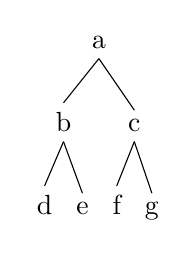
\begin{tikzpicture}
\Tree
[.a     
    [.b
      [.d
      ]
      [.e
      ]
    ]
    [.c
      [.f
      ]
      [.g
      ]
    ]
]
\end{tikzpicture}
\quad \texttt{b2 = }
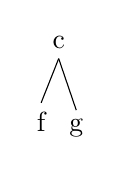
\begin{tikzpicture}
\Tree
[.c
  [.f
  ]
  [.g
  ]
]
\end{tikzpicture}
\quad\texttt{b3 = }
\begin{tikzpicture}
\Tree
[.a
  [.b
    [.d
    ]
    \edge[blank]; \node[blank]{};
  ]
  [.c
  ]
]
\end{tikzpicture}
\quad\texttt{b4 = }
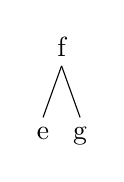
\begin{tikzpicture}
\Tree
[.f
  [.e
  ]
  [.g
  ]
]
\end{tikzpicture} \newline

\begin{center}
\begin{tabbing}
\texttt{b1.isSubtree(b2) $\rightarrow$ true} \quad \quad \quad \= \texttt{b1.isSubtree(b3) $\rightarrow$ true} \\
\texttt{b1.isSubtree(b4) $\rightarrow$ false} \> \texttt{b2.isSubtree(b1) $\rightarrow$ false}
\end{tabbing}
\end{center}

\vspace{4pt}
\noindent You may use the following BinaryTree implementation

\begin{verbatim}
  public class BinaryTree<E>{
    BNode<E> root;
    int size;

    //Nested node class
    private static class BNode<E>{
      BNode<E> left, right;
      E data;
    }
  }
\end{verbatim}

\noindent \textbf{Do not create any new data structures or use any other Java classes or methods.}

\clearpage
\begin{verbatim}
  // Determines whether "other" is a subtree of "this"
  // pre: other != null
  // post: Neither tree is altered by this operation
  public boolean isSubtree(BinaryTree<E> other) {
\end{verbatim}
\end{document}
